\chapter{State of the Art}
\printmyminitoc{1}

Für eine Sicherheitsanalyse von maritimen Steuerungssystemen ist es wichtig, die aktuelle Technik und die
Möglichkeiten von Angreifern zu kennen. In diesem Kapitel wird der aktuelle Stand der Technik vorgestellt.
Der Fokus liegt dabei auf Technologien, die für die Arbeit relevant sind.

\section{Rogue Device}
Unter einem Rogue Device versteht man ein Gerät, das sich unautorisiert und unauffällig in ein Netzwerk integriert \cite{Scarfone2008}.
Dies kann ein Raspberry Pi sein, der sich in ein Netzwerk einbindet und Daten abfängt oder manipuliert. Hierüber können 
sich Angreifer Zugriff auf das Netzwerk verschaffen. 
Ein solches Gerät kann dazu verwendet werden, um eigenen Code auszuführen. Der kann beispielsweise Daten veränden oder 
weitere Angriffe vorbereiten. Zudem kann es von Angreifern aus der Ferne gesteuert werden, wodurch gezielte 
Manipulationen oder Spionageangriffe vereinfacht werden. Darüber hinaus lässt sich ein Rogue Device nutzen, um Informationen 
über das Netzwerk zu sammeln, etwa durch das Mithören von Kommunikation oder die Analyse von Sicherheitsmechanismen.
Das ermöglicht es, Schwachstellen im Netzwerk aufzudecken und gezielt auszunutzen.

\subsection{Angriff mit einem Rogue Device}
Die Idee einen Angriff mit einem Rogue Device durchzuführen, ist nicht neu. Im Jahr 2017 hat Buttigieg et al. \cite{Buttigieg2017}
den möglichen Angriff auf ein automobiles System mit einem Rogue Device untersucht. Bei dem System handelte es sich um einen
CAN-Bus, um das Armaturenbrett eines Fahrzeugs zu steuern. Der weitere Fahrzeugteil wurde in einer Simulation dargestellt.
Buttigieg et al. hat erforscht, ob ein Rogue Device als unautorisiertes 
Gerät in einem CAN-Bus eingebunden werden kann. 
Dazu wurden zuerst die Schwachstellen eines CAN-Bus untersucht. Diese
sind in Abschnitt \ref{sec:canBusVulnerabilities} näher beleuchtet. Es werden zwei verschiedene Angriffe beschrieben.
Der erste Angriff umfasst das Einfügen von bösartigem Code in ein originales Steuergerät. Die zweite Methode ist das Ersetzen
des originalen Steuergerätes durch ein Rogue Device. Die letztere Methode ist für diese Arbeit relevant, da dieser Ansatz
ähnlich ist, wie der in dieser Arbeit verfolgte. Allerdings wurde in der Arbeit von Buttigieg et al. nicht mit einem
J1939-Standard gearbeitet, sondern mit dem ursprünglichen CAN-Standard. Es sollte weiterhin ein Man-in-the-Middle-Angriff
mit dem Rogue Device realisiert werden. \\
Im Ergebnis konnte ein Rogue Device erfolgreich unentdeckt integiert werden. Es konnten manipulierte CAN-Nachrichten gesendet werden.
Die manipulierten Informationen wurden von den Instrumenten dargestellt. Jedoch wurde nicht die Möglichkeit untersucht, manipulierte
Nachrichten an das Motorsteuergerät zu senden.


\section{Arbeit mit dem CAN-Bus}
Die Technologie des CAN-Bus wird in vielen Bereichen eingesetzt.
Daher gibt es auch viele Tools und Bibliotheken, die es ermöglichen, mit dem CAN-Bus zu arbeiten.
In dem folgenden Abschnitt wird der aktuelle Stand der Technik betrachtet.

\subsection{Anbindung von Raspberry Pi an CAN-Bus} \label{sec:raspberryPiToCAN}	
In der folgenden Arbeit soll ein Raspberry Pi an einen CAN-Bus angeschlossen werden. 
Im Folgenden werden einige verschiede Möglichkeiten vorgestellt.\\
Die erste Möglichkeit ist die Verwendung eines Microchip MCP251x, der als CAN-Controller dient \cite{Salunkhe2016}. Dieser wird 
mit dem Microchip MCP2551 ergänzt, der als CAN-Transceiver dient. Diese Kombination ermöglicht es, den
Raspberry Pi mit dem CAN-Bus zu verbinden. Der MCP251x wird über die SPI-Schnittstelle (Serial Peripheral Interface) 
des Raspberry Pi angeschlossen. Dazu wird ein Treiber benötigt, der die Kommunikation zwischen dem Raspberry Pi und dem
MCP251x ermöglicht. Ein solcher Treiber ist bereits seit dem 05.05.2015 im Raspberry Pi OS (ehemals Raspbian OS)
integriert \cite{Salunkhe2016}. 
Um diese Möglichkeit zu vereinfachen, gibt es auch verschiedene HATs (Hardware Attached on Top), die solche Microchips
bereits integriert haben \cite{Pant2019}. Ein Beispiel dafür ist das PiCan2 von SK Pang Electronics. Dieses Board wird auf den 
GPIO-Pins (General Purpose Input/Output) des Raspberry Pi gesteckt. Es erlaubt dem Raspberry Pi mit dem CAN-Bus
zu kommunizieren. Das PiCan2 unterstützt eine Geschwindigkeit von bis zu 1Mbit/s. \\
Es besteht auch die Möglichkeit, einen USB-CAN-Adapter zu verwenden. Damit ist die Anbindung eines 
beliebigen Computer an den CAN-Bus möglich.
Ein Beispiel für einen solchen Adapter ist der UCAN von Fysetc \cite{FysetcUCAN}. 
Die Hardware und Firmware des Adapters
sind open-source. Die Verbindung zum Raspberry Pi erfolgt über USB-C.
Zum CAN-Bus müssen lediglich CAN\_H und CAN\_L und die Masse verbunden werden. Da CAN-Bus Treiber für Linux, Windows und Mac
vorhanden sind, kann der UCAN mit diesen Betriebssystemen verwendet werden. 



\subsection{Übersetzung von CAN-Nachrichten} \label{sec:canTranslation}
Viele Software Tools ermöglichen die Arbeit mit dem CAN-Bus. Diese Tools unterscheiden sich in ihrem Funktionsumfang
und den Anwendungsbereichen.
Einige Programme sind speziell für die Analyse und das Debugging von CAN-Nachrichten 
ausgelegt, während andere umfassende Entwicklungs- und Simulationsmöglichkeiten bieten. Im Folgenden werden die wichtigsten 
Eigenschaften, Einsatzbereiche und Besonderheiten der einzelnen Tools vorgestellt. \\
\begin{itemize}
    \item \textbf{canCommander}\footnote{\href{https://github.com/MatthewKuKanich/CAN_Commander}{CAN Commander} (besucht am 15.02.2025)}: 
    Dieses Tool ermöglicht das Senden und Empfangen von CAN-Nachrichten. Es bietet eine einfache 
    Benutzeroberfläche und umfangreiche Analysefunktionen. Mit canCommander können CAN-Nachrichten aufgezeichnet, 
    analysiert und bearbeitet werden. Dabei können auch Nachrichten gesendet und injiziert werden. Es wird auch eine
    schon vorbereitete Platine verkauft, die es ermöglicht, mit dem CAN-Bus zu arbeiten. Dennoch ist canCommander ein
    open-source Projekt und kann auch auf anderen Plattformen verwendet werden. Diese Plattformen beschränken sich aber
    auf Mikrocontroller, wie Arduino Uno oder 
    ESP32.
    \item \textbf{cantools}\footnote{\href{https://github.com/cantools/cantools/releases}{cantools} (besucht am 15.02.2025)}: 
    Diese Python-Bibliothek ermöglicht es, CAN-Nachrichten zu dekodieren. Mit cantools können 
    CAN-Daten in ein Menschenlesbares Format umgewandelt werden. Die Bibliothek 
    bietet eine Vielzahl von Funktionen und unterstützt verschiedene Protokolle und Datenformate. Damit ist cantools ist ein 
    nützliches Werkzeug für die Analyse und Verarbeitung von CAN-Nachrichten und eignet sich für die Entwicklung von 
    Anwendungen, die mit dem CAN-Bus arbeiten.
    \item \textbf{CANoe}\footnote{\href{https://www.vector.com/de/de/produkte/produkte-a-z/software/canoe/}{CANoe} (besucht am 15.02.2025)}: 
    Dieses eigenständige kommerzielle Tool wurde von der Firma Vector Informatik GmbH. entwickelt.
    Es bietet eine vielzahl an verschiedenen Funktionen. CANoe ermöglicht die Entwicklung, Simulation und Analyse von
    CAN-Netzwerken. Es unterstützt verschiedene Protokolle und 
    Datenformate.
    \item \textbf{can\_decoder}\footnote{\href{https://github.com/CSS-Electronics/can_decoder}{can\_decoder} (besucht am 15.02.2025)}: 
    Das Open-Source-Projekt ermöglicht das Dekodieren von CAN-Nachrichten. Es wurde von der Firma
    CSS-Electronics entwickelt und ist auf GitHub verfügbar. Allerdings ist das Projekt nicht mehr aktiv und wird nicht mehr
    weiterentwickelt. Trotzdem kann es ein nützliches Werkzeug für die Analyse und Verarbeitung von CAN-Nachrichten 
    sein.
    \item \textbf{SavvyCAN}\footnote{\href{https://savvycan.com/index.php}{SavvyCAN} (besucht am 15.02.2025)}: 
    Die C++ Anwendung kann CAN-Nachrichten aufzeichnen, welche zum Reverse-Engineering genutzt werden können.
    Hiermit können auch einzelne Nachrichten dekodiert werden. SavvyCAN ist ein Open-Source-Projekt und kann auf GitHub gefunden werden. 
    Zusätzlich gibt es Unterstützung auf Linux und Windows.
    \item \textbf{can-utils}\footnote{\href{https://github.com/linux-can/can-utils}{can-utils} (besucht am 15.02.2025)}: 
    Diese Set an Linux-Tools ermöglichen die Arbeit mit dem CAN-Bus. Damit ist es möglich, CAN-Nachrichten 
    zu senden und zu empfangen.
    Es ist ein Open-Source-Projekt und kann auf GitHub gefunden werden. Diese Tools bieten eine Grundlage für die Entwicklung von 
    Anwendungen, die mit dem CAN-Bus arbeiten.
\end{itemize}

\subsection{DBC-Dateien}
Es ist essentiell die Nutzlast der CAN-Bus Nachrichten Informationen zuzuordnen. 
Das kann in der Form einer DBC-Datei geschehen\cite{Choi2021}. 
Diese Datei schlüsselt auf, welche Informationen in den verschiedenen CAN-Nachrichten enthalten sind.
Da auch sensible Informationen in den Nachrichten enthalten sein können, wird diese Datei in den meisten 
Fällen nicht öffentlich verfügbar gemacht. Ohne diese Datei können zwar Brute-Force Ansätze verwendet werden,
allerdings ist dies sehr aufwendig und nicht zielführend. \\
Für die Verwendung der Tools, die in Abschnitt \ref{sec:canTranslation} genannt wurden, sind DBC-Dateien notwendig.
Diese werden genutzt, um die zu dekodierenden und kodierenden Nachrichten zu beschreiben. 
Bei \texttt{canCommander}
sind einige DBC-Dateien bereits vorinstalliert. Bei cantools kann die DBC-Datei in das Programm geladen werden.
\begin{figure}[H]
    \centering
    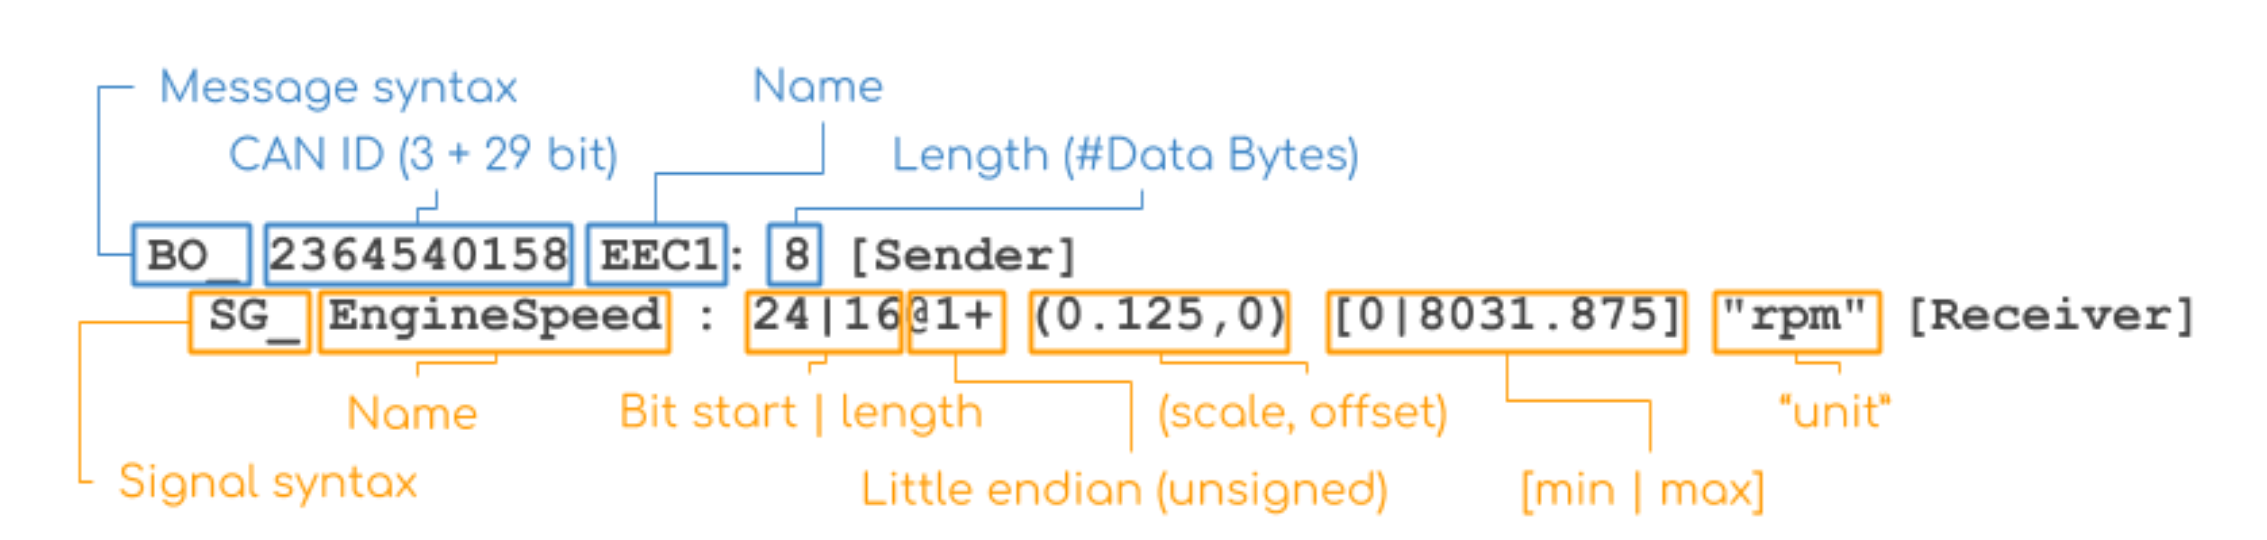
\includegraphics[scale=0.2]{images/CAN-DBC-File-Format-Explained-Intro-Basics_2.png}
    \caption{Auszug aus einer Beispiel DBC-Datei \cite{cssElectronics}}
    \label{fig:dbcfile}
\end{figure}
In Abbildung \ref{fig:dbcfile} ist ein Ausschnitt aus einer DBC-Datei zu sehen.
In dieser sind einzelne Nachrichten aufgelistet. Jede Nachricht hat eine ID, eine Länge und Signale. Diese Signale
haben eine Länge, einen Offset und einen Faktor. Die Signale sind die eigentlichen Informationen, die in den CAN-Nachrichten
kodiert sind. Sie stellen also die Nutzlast der Nachrichten dar. Mit diesen Informationen kann eine Nachricht erstellt werden.
Im Anschluss an die Nachrichtentypen werden in der DBC-Datei für bestimmte Signale die möglichen Eingaben definiert.
Das hilft bei der richtigen Wahl der Eingabe. 